\documentclass{beamer}

\author{门浩}
\title{典型系统与软件的可疑通信行为分析}
\subtitle{毕业设计开题报告}
\institute[计算机科学与技术]{哈尔滨工业大学(威海)计算机科学与技术学院}
\date{2022年12月5日}
\usepackage{hit-style}
\usepackage[minted,fira,siyuan]{hit-extra}

\begin{document}
 
\begin{frame}
    \titlepage
    \begin{figure}[htpb]
        \begin{center}
            
\includegraphics[width=0.2\linewidth]{pic/hitcolor.jpg}
        \end{center}
    \end{figure}
\end{frame}

\begin{frame}
    \tableofcontents[sectionstyle=show,subsectionstyle=show/shaded/hide,subsubsectionstyle=show/shaded/hide]
\end{frame}


\section{课题背景}
\subsection{官方文件}
\begin{frame}{网信办等}
    % \begin{itemize}[<+->] % 当然,除了alert,手动在里面插 \pause 也行
        \begin{itemize}
        \item \href{http://www.cac.gov.cn/2022-09/08/c_1664260384702890.htm}{《互联网弹窗信息推送服务管理规定》}\upcite{互联网弹窗规定2022}
        \item \href{https://www.miit.gov.cn/zwgk/zcwj/wjfb/txy/art/2020/art_ef035831a43142259ccab5a758704747.html}{APP侵害用户权益专项整治工作}
    \end{itemize}
\end{frame}

\subsection{软件情况}
\begin{frame}{恶意软件}
    % \begin{description}[<+->] % 当然,除了alert,手动在里面插 \pause 也行
        \begin{description}
        \item[恶意程序] CNCERT通报下架移动互联网恶意程序达到2075个\upcite{CNCERT2022}(2022年6月)
        \item[软件漏洞] Spring \href{https://spring.io/blog/2022/03/31/spring-framework-rce-early-announcement}{CVE-2022-22965
} 可使攻击者获取目标主机权限(2022年4月)
        \item[软件后门] “即刻PDF阅读器”内置\href{https://www.huorong.cn/info/1660892844878.html}{后门} ,收集用户隐私(2022年8月)
    \end{description}
\end{frame}

\begin{frame}{软件安全}
    % \begin{description}[<+->] % 当然,除了alert,手动在里面插 \pause 也行
        \begin{description}
        \item[关注恶意软件] 病毒、蠕虫、木马、间谍软件、勒索软件、恐吓软件、僵尸程序、后门 \ldots
        \item[关注常用软件] MS Office、WPS、Matlab、CAD、ProE、常用APP \ldots
    \end{description}
\end{frame}


\section{研究现状及存在问题}

\subsection{软件分类}


\begin{frame}{常见操作系统}
    \begin{table}[h]
        \centering
        \begin{tabular}{c|c}
            Microsoft\textsuperscript{\textregistered}  Word & \LaTeX \\
            \hline
            文字处理工具 & 专业排版软件 \\
            容易上手,简单直观 & 容易上手 \\
            所见即所得 & 所见即所想,所想即所得 \\
            高级功能不易掌握 & 进阶难,但一般用不到 \\
            处理长文档需要丰富经验 & 和短文档处理基本无异 \\
            花费大量时间调格式 & 无需担心格式,专心作者内容 \\
            公式排版差强人意 & 尤其擅长公式排版 \\
            二进制格式,兼容性差 & 文本文件,易读、稳定 \\
            付费商业许可 & 自由免费使用 \\
        \end{tabular}
    \end{table}
\end{frame}

\begin{frame}{常见通用及专业软件}
    \begin{table}[h]
        \centering
        \begin{tabular}{c|c}
            Microsoft\textsuperscript{\textregistered}  Word & \LaTeX \\
            \hline
            文字处理工具 & 专业排版软件 \\
            容易上手,简单直观 & 容易上手 \\
            所见即所得 & 所见即所想,所想即所得 \\
            高级功能不易掌握 & 进阶难,但一般用不到 \\
            处理长文档需要丰富经验 & 和短文档处理基本无异 \\
            花费大量时间调格式 & 无需担心格式,专心作者内容 \\
            公式排版差强人意 & 尤其擅长公式排版 \\
            二进制格式,兼容性差 & 文本文件,易读、稳定 \\
            付费商业许可 & 自由免费使用 \\
        \end{tabular}
    \end{table}
\end{frame}


\section{研究内容}

\subsection{美化主题}

\begin{frame}{这一份主题与 THU Beamer Theme 区别在于}
    \begin{itemize}
        \item 全文使用无衬线体, 中文使用思源黑体, 英文使用 FiraGO, 公式使用 unicode-math 搭配 Fira Math 字体. 下载及使用方法请看  \href{https://github.com/syvshc/HITBeamer\#readme}{README}
        \item 修改了颜色为我也不知道应该叫什么的颜色
        \item 校徽改为了哈工大校徽
        \item 放弃了不显示小标题的 \href{https://github.com/Trinkle23897/THU-Beamer-Theme/commit/061f088d1c7e4b2d2f1f581f3745945ecbb63f25}{commit}, 如果有需要请自行按照该 commit 修改 \mintinline{text}{HIT.sty}
    \end{itemize}
\end{frame}

\subsection{如何更好地做Beamer}

\begin{frame}{Why Beamer}
    \begin{itemize}
        \item \LaTeX 广泛用于学术界,期刊会议论文模板
    \end{itemize}
    \begin{table}[h]
        \centering
        \begin{tabular}{c|c}
            Microsoft\textsuperscript{\textregistered}  Word & \LaTeX \\
            \hline
            文字处理工具 & 专业排版软件 \\
            容易上手,简单直观 & 容易上手 \\
            所见即所得 & 所见即所想,所想即所得 \\
            高级功能不易掌握 & 进阶难,但一般用不到 \\
            处理长文档需要丰富经验 & 和短文档处理基本无异 \\
            花费大量时间调格式 & 无需担心格式,专心作者内容 \\
            公式排版差强人意 & 尤其擅长公式排版 \\
            二进制格式,兼容性差 & 文本文件,易读、稳定 \\
            付费商业许可 & 自由免费使用 \\
        \end{tabular}
    \end{table}
\end{frame}

\begin{frame}{排版举例}
    \begin{exampleblock}{无编号公式} % 加 * 
        \begin{equation*}
            J(\theta) = \mathbb{E}_{\pi_\theta}[G_t] = \sum_{s\in\mathcal{S}} d^\pi (s)V^\pi(s)=\sum_{s\in\mathcal{S}} d^\pi(s)\sum_{a\in\mathcal{A}}\pi_\theta(a|s)Q^\pi(s,a)
        \end{equation*}
    \end{exampleblock}
    \begin{exampleblock}{多行多列公式\footnote{如果公式中有文字出现,请用 $\backslash$mathrm\{\} 或者 $\backslash$text\{\} 包含,不然就会变成 $clip$,在公式里看起来比 $\mathrm{clip}$ 丑非常多。}}
        % 使用 & 分隔
        \begin{align}
            Q_\mathrm{target}&=r+\gamma Q^\pi(s^\prime, \pi_\theta(s^\prime)+\epsilon)\\
            \epsilon&\sim\mathrm{clip}(\mathcal{N}(0, \sigma), -c, c)\nonumber
        \end{align}
    \end{exampleblock}
\end{frame}

\begin{frame}
    \begin{exampleblock}{编号多行公式}
        % Taken from Mathmode.tex
        \begin{multline}
            A=\lim_{n\rightarrow\infty}\Delta x\left(a^{2}+\left(a^{2}+2a\Delta x+\left(\Delta x\right)^{2}\right)\right.\label{eq:reset}\\
            +\left(a^{2}+2\cdot2a\Delta x+2^{2}\left(\Delta x\right)^{2}\right)\\
            +\left(a^{2}+2\cdot3a\Delta x+3^{2}\left(\Delta x\right)^{2}\right)\\
            +\ldots\\
            \left.+\left(a^{2}+2\cdot(n-1)a\Delta x+(n-1)^{2}\left(\Delta x\right)^{2}\right)\right)\\
            =\frac{1}{3}\left(b^{3}-a^{3}\right)
        \end{multline}
    \end{exampleblock}
\end{frame}

\begin{frame}{图形与分栏}
    % From thuthesis user guide.
    \begin{minipage}[c]{0.3\linewidth}
        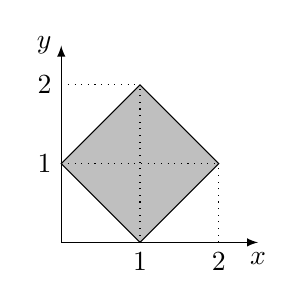
\begin{tikzpicture}
            \draw[-latex] (0, 0) -- (2.5, 0) node[below] {$ x $};
            \draw[-latex] (0, 0) -- (0, 2.5) node[left] {$ y $};
            \draw[fill=gray!50] (0, 1) -- (1, 2) -- (2, 1) -- (1, 0) -- cycle;
            \draw[dotted] (0, 2) node[left] {$ 2 $} -- (1, 2);
            \draw[dotted] (0, 1) node[left] {$ 1 $} -- (2, 1);
            \draw[dotted] (1, 0) node[below] {$ 1 $} -- (1, 2);
            \draw[dotted] (2, 0) node[below] {$ 2 $} -- (2, 1);
        \end{tikzpicture}
    \end{minipage}\hspace{1cm}
    \begin{minipage}{0.5\linewidth}
        \medskip
        %\hspace{2cm}
        \begin{figure}[h]
            \centering
            \includegraphics[height=.4\textheight]{pic/dtmf.pdf}
        \end{figure}
    \end{minipage}
\end{frame}

\begin{frame}[fragile]{\LaTeX{} 常用命令}
    \begin{exampleblock}{命令}
        \centering
        \small
        \begin{tabular}{llll}
            \cmd{chapter} & \cmd{section} & \cmd{subsection} & \cmd{paragraph} \\
            章 & 节 & 小节 & 带题头段落 \\\hline
            \cmd{centering} & \cmd{emph} & \cmd{verb} & \cmd{url} \\
            居中对齐 & 强调 & 抄录命令 & 超链接 \\\hline
            \cmd{footnote} & \cmd{item} & \cmd{caption} & \cmd{includegraphics} \\
            脚注 & 列表条目 & 标题 & 插入图片 \\\hline
            \cmd{label} & \cmd{cite} & \cmd{ref} \\
            标号 & 引用参考文献 & 引用图表公式等\\\hline
        \end{tabular}
    \end{exampleblock}
    \begin{exampleblock}{环境}
        \centering
        \small
        \begin{tabular}{lll}\hline
            \env{table} & \env{figure} & \env{equation}\\
            表格 & 图片 & 公式 \\\hline
            \env{itemize} & \env{enumerate} & \env{description}\\
            无编号列表 & 编号列表 & 描述 \\\hline
        \end{tabular}
    \end{exampleblock}
\end{frame}

\begin{frame}[fragile]{\LaTeX{} 环境命令举例}
    \begin{minipage}{0.5\linewidth}
\begin{minted}{latex}
\begin{itemize}
  \item A \item B
  \item C
  \begin{itemize}
    \item C-1
  \end{itemize}
\end{itemize}
\end{minted}
    \end{minipage}\hspace{1cm}
    \begin{minipage}{0.3\linewidth}
        \begin{itemize}
            \item A
            \item B
            \item C
            \begin{itemize}
                \item C-1
            \end{itemize}
        \end{itemize}
    \end{minipage}
    \medskip
    \pause
    \begin{minipage}{0.5\linewidth}
        这是 \env{minted} 环境的示例
\begin{minted}{latex}
\begin{enumerate}
  \item 巨佬 \item 大佬
  \item 萌新
  \begin{itemize}
    \item[n+e] 瑟瑟发抖
  \end{itemize}
\end{enumerate}
\end{minted}
    \end{minipage}\hspace{1cm}
    \begin{minipage}{0.3\linewidth}
        \begin{enumerate}
            \item 巨佬
            \item 大佬
            \item 萌新
            \begin{itemize}
                \item[n+e] 瑟瑟发抖
            \end{itemize}
        \end{enumerate}
    \end{minipage}
\end{frame}

\begin{frame}[fragile]{\LaTeX{} 数学公式}
    \begin{columns}
        \begin{column}{.55\textwidth}
            这是 \env{lstlisting} 环境的示例
\begin{lstlisting}[language=TeX]
$V = \frac{4}{3}\pi r^3$

\[
  V = \frac{4}{3}\pi r^3
\]

\begin{equation}
  \label{eq:vsphere}
  V = \frac{4}{3}\pi r^3
\end{equation}
\end{lstlisting}
        \end{column}
        \begin{column}{.4\textwidth}
            $V = \frac{4}{3}\pi r^3$
            \[
                V = \frac{4}{3}\pi r^3
            \]
            \begin{equation}
                \label{eq:vsphere}
                V = \frac{4}{3}\pi r^3
            \end{equation}
        \end{column}
    \end{columns}
    \begin{itemize}
        \item 更多内容请看 \href{https://zh.wikipedia.org/wiki/Help:数学公式}{\color{purple}{这里}}
    \end{itemize}
\end{frame}

\begin{frame}[fragile]
    \begin{columns}
        \column{.5\textwidth}
\begin{minted}{latex}
    \begin{table}[htbp]
      \caption{编号与含义}
      \label{tab:number}
      \centering
      \begin{tabular}{cl}
        \toprule
        编号 & 含义 \\
        \midrule
        1 & 4.0 \\
        2 & 3.7 \\
        \bottomrule
      \end{tabular}
    \end{table}
    公式~(\ref{eq:vsphere}) 的编号与含义请参见表~\ref{tab:number}。
\end{minted}
        \column{.4\textwidth}
        \begin{table}[htpb]
            \centering
            \caption{编号与含义}
            \label{tab:number}
            \begin{tabular}{cl}\toprule
                编号 & 含义 \\\midrule
                1 & 4.0\\
                2 & 3.7\\\bottomrule
            \end{tabular}
        \end{table}
        \normalsize 公式~(\ref{eq:vsphere})的编号与含义请参见表~\ref{tab:number}。
    \end{columns}
\end{frame}

\begin{frame}[fragile]{minted 环境 与 python 代码}
    \begin{minted}[]{python}
        import numpy as np
        print("Hello World")
        np.array([x for x in range(5) if x % 2 == 1])
    \end{minted}
\end{frame}

\begin{frame}{作图}
    \begin{itemize}
        \item 矢量图 eps, ps, pdf
        \begin{itemize}
            \item METAPOST, pstricks, pgf $\ldots$
            \item Xfig, Dia, Visio, Inkscape $\ldots$
            \item Matlab / Excel 等保存为 pdf
        \end{itemize}
        \item 标量图 png, jpg, tiff $\ldots$
        \begin{itemize}
            \item 提高清晰度,避免发虚
            \item 应尽量避免使用
        \end{itemize}
    \end{itemize}
    \begin{figure}[htpb]
        \centering
        \includegraphics[width=0.2\linewidth]{pic/hitlogo.pdf}
        \caption{\CJKsout{这个校徽就不是矢量图, 差评. }现在这个是矢量图了\footnote{从 \url{http://100.hit.edu.cn/xqgwsy/xqbs} 这里的 VIS 中扒下来的}}
    \end{figure}
    
\end{frame}

\begin{frame}{定理环境与块环境}
    \begin{definition}[数列极限]
        对任意 $ \varepsilon>0 $, 存在 $ N\in\symbb{N} $, 使得当 $ n>N $ 时, 有
        \[
            \abs{a_{n}-a}<\varepsilon
        \]   
        那么我们称数列 $ \qty{a_{n}} $ \emph{收敛}, 记为
        \[
            \lim_{n\to\infty}a_{n}=a.
        \]
    \end{definition}
    \begin{block}{注}
        可使用的定理环境为 \env{theorem}, \env{corollary}, \env{definition}, \env{definitions}, \env{fact}, \env{example}, 与 \env{examples}  
    \end{block}
\end{frame}


\section{待解决问题及方案}
\begin{frame}
    \begin{itemize}
        \item 一月:完成文献调研
        \item 二月:复现并评测各种Beamer主题美观程度
        \item 三、四月:美化HIT Beamer主题
        \item 五月:论文撰写
    \end{itemize}
    \nocite{*}
\end{frame}


\section{计划进度}
\begin{frame}
    \begin{itemize}
        \item 一月:完成文献调研
        \item 二月:复现并评测各种Beamer主题美观程度
        \item 三、四月:美化HIT Beamer主题
        \item 五月:论文撰写
    \end{itemize}
    \nocite{*}
\end{frame}


\section{参考文献}

\begin{frame}[allowframebreaks]
    % \bibliographystyle{hithesis}
    % 如果参考文献太多的话,可以像下面这样调整字体:
    \tiny\bibliographystyle{hithesis}
    \bibliography{ref}
\end{frame}
 
\begin{frame}
    \begin{center}
        {\Huge\calligra Thanks!}
    \end{center}
\end{frame}

\end{document}